% Include with % Include with % Include with % Include with \input{figure_floats} from a PNAS manuscript in paper_simple.
% Plot PDFs contain no manuscript captions; all caption prose is typeset here.
\begin{figure*}[!t]
  \centering
  \includegraphics[trim=8bp 30bp 5bp 10bp,clip,width=0.91\textwidth]{../output/backbone_h1_findings/combined_before_rotation_2026-11-24.pdf}
  \caption{\textbf{Transfer-network structure and Premier League entry by age, recorded seasons 2012/13--2024/25.} Both panels use the same sample of 16,636 eligible transfers involving 4,602 players. \textbf{(a)} The directed disparity backbone at $\alpha = 0.20$ retains 383 clubs and 1,396 routes carrying 5,271 transfers (31.7\% of the sample). Routes are retained when their disparity score is below $\alpha$ at either eligible endpoint. This is an exploratory local filter. Colours and shapes identify five Louvain communities. Each community is named after its member club with the highest total degree before disparity filtering. Arrows point from origin to destination, and line width increases with transfer count. Node area increases with the square root of each club's total incoming and outgoing transfer count before filtering. The network pools both age groups and includes Premier League and other destinations. \textbf{(b)} Using the full sample, Premier League joining rates were 12.14\% for transfers involving players aged 30+ (129/1,063) and 14.56\% for those under 30 (2,267/15,573), an older-minus-younger gap of $-2.42$ percentage points. The histogram shows 999 age-label shuffles within origin club and recorded season, with a mean gap of $-1.31$ points. The legend's $\pm0.83$ denotes one standard deviation of the shuffled gaps; the fitted normal curve is illustrative. The empirical one-sided p-value is 0.098, providing limited evidence against this conditional null.}
  \label{fig:entry-age}
\end{figure*}

\begin{figure*}[!t]
  \centering
  \begin{minipage}[t]{0.47\textwidth}
    \vspace{0pt}
    \centering
    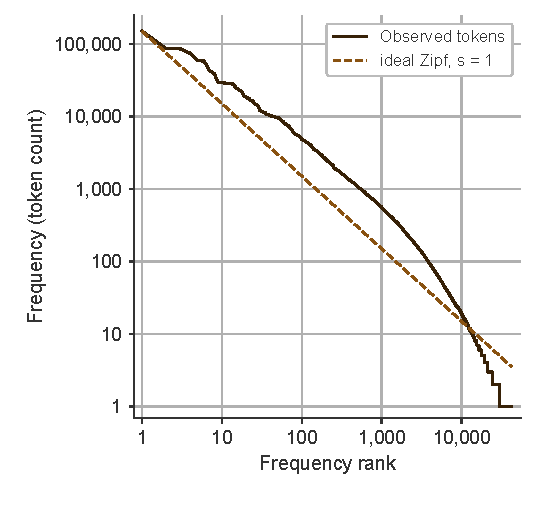
\includegraphics[trim=0bp 13bp 0bp 4bp,clip,width=\linewidth]{../reruns/h1_2012_13-2024_25/output/guardian_text_description_findings/rank_frequency_loglog.pdf}
    \caption{\textbf{Token rank and frequency in the selected Guardian corpus.} Both axes are logarithmic. Counts include stopwords. The ideal Zipf reference divides the most frequent token's count by rank.}
    \label{fig:guardian-rank-frequency}
  \end{minipage}\hfill
  \begin{minipage}[t]{0.50\textwidth}
    \vspace{0pt}
    \centering
    \captionof{table}{Ten most frequent tokens in the selected Guardian corpus, with and without stopwords.}
    \label{tab:guardian-tokens}
    \setlength{\tabcolsep}{3pt}
    \begin{tabular}{@{}rlrrlrr@{}}
      \toprule
      & \multicolumn{3}{c}{With stopwords} & \multicolumn{3}{c}{Without stopwords}\\
      \cmidrule(lr){2-4}\cmidrule(l){5-7}
      Rank & Token & Count & \% & Token & Count & \%\\
      \midrule
      1 & the & 150,246 & 3.9 & season & 17,521 & 0.8\\
      2 & and & 86,037 & 2.2 & \pounds & 15,740 & 0.7\\
      3 & to & 85,471 & 2.2 & m & 14,903 & 0.6\\
      4 & a & 74,360 & 1.9 & city & 11,627 & 0.5\\
      5 & in & 58,569 & 1.5 & united & 11,265 & 0.5\\
      6 & of & 58,167 & 1.5 & chelsea & 10,557 & 0.5\\
      7 & \textquoteright{}s & 42,517 & 1.1 & unknown & 10,439 & 0.4\\
      8 & for & 39,181 & 1.0 & manchester & 10,280 & 0.4\\
      9 & his & 29,501 & 0.8 & form & 10,093 & 0.4\\
      10 & is & 29,321 & 0.8 & injured & 9,960 & 0.4\\
      \bottomrule
    \end{tabular}

    \addtabletext{Percentages use the token total for each ranking (3,870,272 with stopwords and 2,336,122 without stopwords). Both rankings exclude punctuation and whitespace.}
  \end{minipage}
\end{figure*}

% Schedule the monthly plot with the tone-change Results.
\newcommand{\guardianSentimentFigure}{%
\begin{figure*}[!t]
  \centering
  \includegraphics[trim=10bp 8bp 0bp 5bp,clip,width=0.83\textwidth]{../output/h2_monthly_period_means_findings/combined.pdf}
  \caption{\textbf{Guardian sentiment before and after Premier League signings, by age and scoring method.} Panels show RoBERTa (main instrument), VADER, Bing, and Bing excluding 21 football-related words. Higher scores indicate more positive language. Orange identifies signings involving players aged 30+; dark brown identifies those under 30. The sample contains 820 signings (67 older, 753 younger), each with at least five scored sentences in both periods: days $-365$ to $-8$ before signing and +8 to +365 after signing. Liveblogs and match reports are excluded.\endgraf
Curves show monthly sentence scores averaged first within each signing and then across contributing signings, smoothed with a centred three-month moving average separately before and after signing. Monthly membership varies with available coverage. The dashed line marks the signing date. Dots show age-group means of signing-level period means, giving each signing equal weight. Their positions at $-6$ and +6 months are for display; the short horizontal segments are fixed markers. No uncertainty intervals are shown. These period means are calculated separately from the smoothed curves.\endgraf
The main RoBERTa comparison estimates an older-minus-younger difference in before-to-after changes of +0.0060 score units (two-sided p = 0.7558; 5,000 age-label shuffles within signing season). This provides no clear evidence of different changes by age, with limited sensitivity to smaller differences.}
  \label{fig:h2-monthly-tone}
\end{figure*}
}
 from a PNAS manuscript in paper_simple.
% Plot PDFs contain no manuscript captions; all caption prose is typeset here.
\begin{figure*}[!t]
  \centering
  \includegraphics[trim=8bp 30bp 5bp 10bp,clip,width=0.91\textwidth]{../output/backbone_h1_findings/combined_before_rotation_2026-11-24.pdf}
  \caption{\textbf{Transfer-network structure and Premier League entry by age, recorded seasons 2012/13--2024/25.} Both panels use the same sample of 16,636 eligible transfers involving 4,602 players. \textbf{(a)} The directed disparity backbone at $\alpha = 0.20$ retains 383 clubs and 1,396 routes carrying 5,271 transfers (31.7\% of the sample). Routes are retained when their disparity score is below $\alpha$ at either eligible endpoint. This is an exploratory local filter. Colours and shapes identify five Louvain communities. Each community is named after its member club with the highest total degree before disparity filtering. Arrows point from origin to destination, and line width increases with transfer count. Node area increases with the square root of each club's total incoming and outgoing transfer count before filtering. The network pools both age groups and includes Premier League and other destinations. \textbf{(b)} Using the full sample, Premier League joining rates were 12.14\% for transfers involving players aged 30+ (129/1,063) and 14.56\% for those under 30 (2,267/15,573), an older-minus-younger gap of $-2.42$ percentage points. The histogram shows 999 age-label shuffles within origin club and recorded season, with a mean gap of $-1.31$ points. The legend's $\pm0.83$ denotes one standard deviation of the shuffled gaps; the fitted normal curve is illustrative. The empirical one-sided p-value is 0.098, providing limited evidence against this conditional null.}
  \label{fig:entry-age}
\end{figure*}

\begin{figure*}[!t]
  \centering
  \begin{minipage}[t]{0.47\textwidth}
    \vspace{0pt}
    \centering
    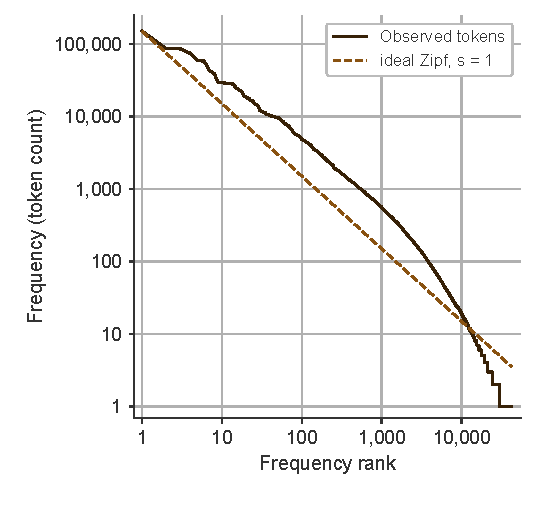
\includegraphics[trim=0bp 13bp 0bp 4bp,clip,width=\linewidth]{../reruns/h1_2012_13-2024_25/output/guardian_text_description_findings/rank_frequency_loglog.pdf}
    \caption{\textbf{Token rank and frequency in the selected Guardian corpus.} Both axes are logarithmic. Counts include stopwords. The ideal Zipf reference divides the most frequent token's count by rank.}
    \label{fig:guardian-rank-frequency}
  \end{minipage}\hfill
  \begin{minipage}[t]{0.50\textwidth}
    \vspace{0pt}
    \centering
    \captionof{table}{Ten most frequent tokens in the selected Guardian corpus, with and without stopwords.}
    \label{tab:guardian-tokens}
    \setlength{\tabcolsep}{3pt}
    \begin{tabular}{@{}rlrrlrr@{}}
      \toprule
      & \multicolumn{3}{c}{With stopwords} & \multicolumn{3}{c}{Without stopwords}\\
      \cmidrule(lr){2-4}\cmidrule(l){5-7}
      Rank & Token & Count & \% & Token & Count & \%\\
      \midrule
      1 & the & 150,246 & 3.9 & season & 17,521 & 0.8\\
      2 & and & 86,037 & 2.2 & \pounds & 15,740 & 0.7\\
      3 & to & 85,471 & 2.2 & m & 14,903 & 0.6\\
      4 & a & 74,360 & 1.9 & city & 11,627 & 0.5\\
      5 & in & 58,569 & 1.5 & united & 11,265 & 0.5\\
      6 & of & 58,167 & 1.5 & chelsea & 10,557 & 0.5\\
      7 & \textquoteright{}s & 42,517 & 1.1 & unknown & 10,439 & 0.4\\
      8 & for & 39,181 & 1.0 & manchester & 10,280 & 0.4\\
      9 & his & 29,501 & 0.8 & form & 10,093 & 0.4\\
      10 & is & 29,321 & 0.8 & injured & 9,960 & 0.4\\
      \bottomrule
    \end{tabular}

    \addtabletext{Percentages use the token total for each ranking (3,870,272 with stopwords and 2,336,122 without stopwords). Both rankings exclude punctuation and whitespace.}
  \end{minipage}
\end{figure*}

% Schedule the monthly plot with the tone-change Results.
\newcommand{\guardianSentimentFigure}{%
\begin{figure*}[!t]
  \centering
  \includegraphics[trim=10bp 8bp 0bp 5bp,clip,width=0.83\textwidth]{../output/h2_monthly_period_means_findings/combined.pdf}
  \caption{\textbf{Guardian sentiment before and after Premier League signings, by age and scoring method.} Panels show RoBERTa (main instrument), VADER, Bing, and Bing excluding 21 football-related words. Higher scores indicate more positive language. Orange identifies signings involving players aged 30+; dark brown identifies those under 30. The sample contains 820 signings (67 older, 753 younger), each with at least five scored sentences in both periods: days $-365$ to $-8$ before signing and +8 to +365 after signing. Liveblogs and match reports are excluded.\endgraf
Curves show monthly sentence scores averaged first within each signing and then across contributing signings, smoothed with a centred three-month moving average separately before and after signing. Monthly membership varies with available coverage. The dashed line marks the signing date. Dots show age-group means of signing-level period means, giving each signing equal weight. Their positions at $-6$ and +6 months are for display; the short horizontal segments are fixed markers. No uncertainty intervals are shown. These period means are calculated separately from the smoothed curves.\endgraf
The main RoBERTa comparison estimates an older-minus-younger difference in before-to-after changes of +0.0060 score units (two-sided p = 0.7558; 5,000 age-label shuffles within signing season). This provides no clear evidence of different changes by age, with limited sensitivity to smaller differences.}
  \label{fig:h2-monthly-tone}
\end{figure*}
}
 from a PNAS manuscript in paper_simple.
% Plot PDFs contain no manuscript captions; all caption prose is typeset here.
\begin{figure*}[!t]
  \centering
  \includegraphics[trim=8bp 30bp 5bp 10bp,clip,width=0.91\textwidth]{../output/backbone_h1_findings/combined_before_rotation_2026-11-24.pdf}
  \caption{\textbf{Transfer-network structure and Premier League entry by age, recorded seasons 2012/13--2024/25.} Both panels use the same sample of 16,636 eligible transfers involving 4,602 players. \textbf{(a)} The directed disparity backbone at $\alpha = 0.20$ retains 383 clubs and 1,396 routes carrying 5,271 transfers (31.7\% of the sample). Routes are retained when their disparity score is below $\alpha$ at either eligible endpoint. This is an exploratory local filter. Colours and shapes identify five Louvain communities. Each community is named after its member club with the highest total degree before disparity filtering. Arrows point from origin to destination, and line width increases with transfer count. Node area increases with the square root of each club's total incoming and outgoing transfer count before filtering. The network pools both age groups and includes Premier League and other destinations. \textbf{(b)} Using the full sample, Premier League joining rates were 12.14\% for transfers involving players aged 30+ (129/1,063) and 14.56\% for those under 30 (2,267/15,573), an older-minus-younger gap of $-2.42$ percentage points. The histogram shows 999 age-label shuffles within origin club and recorded season, with a mean gap of $-1.31$ points. The legend's $\pm0.83$ denotes one standard deviation of the shuffled gaps; the fitted normal curve is illustrative. The empirical one-sided p-value is 0.098, providing limited evidence against this conditional null.}
  \label{fig:entry-age}
\end{figure*}

\begin{figure*}[!t]
  \centering
  \begin{minipage}[t]{0.47\textwidth}
    \vspace{0pt}
    \centering
    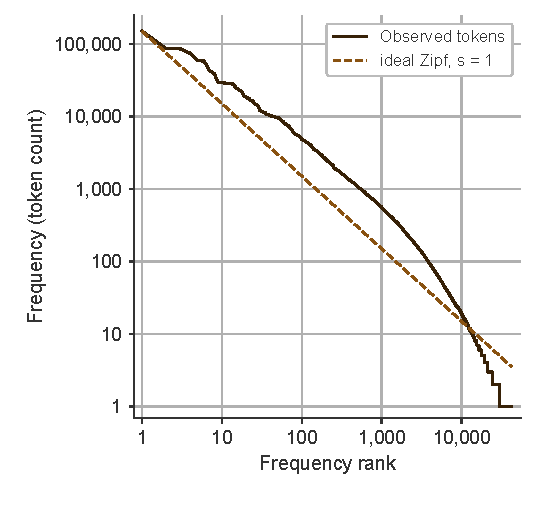
\includegraphics[trim=0bp 13bp 0bp 4bp,clip,width=\linewidth]{../reruns/h1_2012_13-2024_25/output/guardian_text_description_findings/rank_frequency_loglog.pdf}
    \caption{\textbf{Token rank and frequency in the selected Guardian corpus.} Both axes are logarithmic. Counts include stopwords. The ideal Zipf reference divides the most frequent token's count by rank.}
    \label{fig:guardian-rank-frequency}
  \end{minipage}\hfill
  \begin{minipage}[t]{0.50\textwidth}
    \vspace{0pt}
    \centering
    \captionof{table}{Ten most frequent tokens in the selected Guardian corpus, with and without stopwords.}
    \label{tab:guardian-tokens}
    \setlength{\tabcolsep}{3pt}
    \begin{tabular}{@{}rlrrlrr@{}}
      \toprule
      & \multicolumn{3}{c}{With stopwords} & \multicolumn{3}{c}{Without stopwords}\\
      \cmidrule(lr){2-4}\cmidrule(l){5-7}
      Rank & Token & Count & \% & Token & Count & \%\\
      \midrule
      1 & the & 150,246 & 3.9 & season & 17,521 & 0.8\\
      2 & and & 86,037 & 2.2 & \pounds & 15,740 & 0.7\\
      3 & to & 85,471 & 2.2 & m & 14,903 & 0.6\\
      4 & a & 74,360 & 1.9 & city & 11,627 & 0.5\\
      5 & in & 58,569 & 1.5 & united & 11,265 & 0.5\\
      6 & of & 58,167 & 1.5 & chelsea & 10,557 & 0.5\\
      7 & \textquoteright{}s & 42,517 & 1.1 & unknown & 10,439 & 0.4\\
      8 & for & 39,181 & 1.0 & manchester & 10,280 & 0.4\\
      9 & his & 29,501 & 0.8 & form & 10,093 & 0.4\\
      10 & is & 29,321 & 0.8 & injured & 9,960 & 0.4\\
      \bottomrule
    \end{tabular}

    \addtabletext{Percentages use the token total for each ranking (3,870,272 with stopwords and 2,336,122 without stopwords). Both rankings exclude punctuation and whitespace.}
  \end{minipage}
\end{figure*}

% Schedule the monthly plot with the tone-change Results.
\newcommand{\guardianSentimentFigure}{%
\begin{figure*}[!t]
  \centering
  \includegraphics[trim=10bp 8bp 0bp 5bp,clip,width=0.83\textwidth]{../output/h2_monthly_period_means_findings/combined.pdf}
  \caption{\textbf{Guardian sentiment before and after Premier League signings, by age and scoring method.} Panels show RoBERTa (main instrument), VADER, Bing, and Bing excluding 21 football-related words. Higher scores indicate more positive language. Orange identifies signings involving players aged 30+; dark brown identifies those under 30. The sample contains 820 signings (67 older, 753 younger), each with at least five scored sentences in both periods: days $-365$ to $-8$ before signing and +8 to +365 after signing. Liveblogs and match reports are excluded.\endgraf
Curves show monthly sentence scores averaged first within each signing and then across contributing signings, smoothed with a centred three-month moving average separately before and after signing. Monthly membership varies with available coverage. The dashed line marks the signing date. Dots show age-group means of signing-level period means, giving each signing equal weight. Their positions at $-6$ and +6 months are for display; the short horizontal segments are fixed markers. No uncertainty intervals are shown. These period means are calculated separately from the smoothed curves.\endgraf
The main RoBERTa comparison estimates an older-minus-younger difference in before-to-after changes of +0.0060 score units (two-sided p = 0.7558; 5,000 age-label shuffles within signing season). This provides no clear evidence of different changes by age, with limited sensitivity to smaller differences.}
  \label{fig:h2-monthly-tone}
\end{figure*}
}
 from a PNAS manuscript in paper_simple.
% Plot PDFs contain no manuscript captions; all caption prose is typeset here.
\begin{figure*}[!t]
  \centering
  \includegraphics[trim=8bp 30bp 5bp 10bp,clip,width=0.91\textwidth]{../output/backbone_h1_findings/combined_before_rotation_2026-11-24.pdf}
  \caption{\textbf{Transfer-network structure and Premier League entry by age, recorded seasons 2012/13--2024/25.} Both panels use the same sample of 16,636 eligible transfers involving 4,602 players. \textbf{(a)} The directed disparity backbone at $\alpha = 0.20$ retains 383 clubs and 1,396 routes carrying 5,271 transfers (31.7\% of the sample). Routes are retained when their disparity score is below $\alpha$ at either eligible endpoint. This is an exploratory local filter. Colours and shapes identify five Louvain communities. Each community is named after its member club with the highest total degree before disparity filtering. Arrows point from origin to destination, and line width increases with transfer count. Node area increases with the square root of each club's total incoming and outgoing transfer count before filtering. The network pools both age groups and includes Premier League and other destinations. \textbf{(b)} Using the full sample, Premier League joining rates were 12.14\% for transfers involving players aged 30+ (129/1,063) and 14.56\% for those under 30 (2,267/15,573), an older-minus-younger gap of $-2.42$ percentage points. The histogram shows 999 age-label shuffles within origin club and recorded season, with a mean gap of $-1.31$ points. The legend's $\pm0.83$ denotes one standard deviation of the shuffled gaps; the fitted normal curve is illustrative. The empirical one-sided p-value is 0.098, providing limited evidence against this conditional null.}
  \label{fig:entry-age}
\end{figure*}

\begin{figure*}[!t]
  \centering
  \begin{minipage}[t]{0.47\textwidth}
    \vspace{0pt}
    \centering
    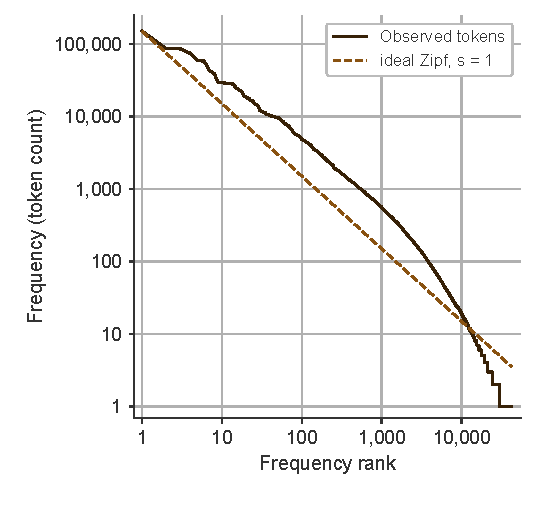
\includegraphics[trim=0bp 13bp 0bp 4bp,clip,width=\linewidth]{../reruns/h1_2012_13-2024_25/output/guardian_text_description_findings/rank_frequency_loglog.pdf}
    \caption{\textbf{Token rank and frequency in the selected Guardian corpus.} Both axes are logarithmic. Counts include stopwords. The ideal Zipf reference divides the most frequent token's count by rank.}
    \label{fig:guardian-rank-frequency}
  \end{minipage}\hfill
  \begin{minipage}[t]{0.50\textwidth}
    \vspace{0pt}
    \centering
    \captionof{table}{Ten most frequent tokens in the selected Guardian corpus, with and without stopwords.}
    \label{tab:guardian-tokens}
    \setlength{\tabcolsep}{3pt}
    \begin{tabular}{@{}rlrrlrr@{}}
      \toprule
      & \multicolumn{3}{c}{With stopwords} & \multicolumn{3}{c}{Without stopwords}\\
      \cmidrule(lr){2-4}\cmidrule(l){5-7}
      Rank & Token & Count & \% & Token & Count & \%\\
      \midrule
      1 & the & 150,246 & 3.9 & season & 17,521 & 0.8\\
      2 & and & 86,037 & 2.2 & \pounds & 15,740 & 0.7\\
      3 & to & 85,471 & 2.2 & m & 14,903 & 0.6\\
      4 & a & 74,360 & 1.9 & city & 11,627 & 0.5\\
      5 & in & 58,569 & 1.5 & united & 11,265 & 0.5\\
      6 & of & 58,167 & 1.5 & chelsea & 10,557 & 0.5\\
      7 & \textquoteright{}s & 42,517 & 1.1 & unknown & 10,439 & 0.4\\
      8 & for & 39,181 & 1.0 & manchester & 10,280 & 0.4\\
      9 & his & 29,501 & 0.8 & form & 10,093 & 0.4\\
      10 & is & 29,321 & 0.8 & injured & 9,960 & 0.4\\
      \bottomrule
    \end{tabular}

    \addtabletext{Percentages use the token total for each ranking (3,870,272 with stopwords and 2,336,122 without stopwords). Both rankings exclude punctuation and whitespace.}
  \end{minipage}
\end{figure*}

% Schedule the monthly plot with the tone-change Results.
\newcommand{\guardianSentimentFigure}{%
\begin{figure*}[!t]
  \centering
  \includegraphics[trim=10bp 8bp 0bp 5bp,clip,width=0.83\textwidth]{../output/h2_monthly_period_means_findings/combined.pdf}
  \caption{\textbf{Guardian sentiment before and after Premier League signings, by age and scoring method.} Panels show RoBERTa (main instrument), VADER, Bing, and Bing excluding 21 football-related words. Higher scores indicate more positive language. Orange identifies signings involving players aged 30+; dark brown identifies those under 30. The sample contains 820 signings (67 older, 753 younger), each with at least five scored sentences in both periods: days $-365$ to $-8$ before signing and +8 to +365 after signing. Liveblogs and match reports are excluded.\endgraf
Curves show monthly sentence scores averaged first within each signing and then across contributing signings, smoothed with a centred three-month moving average separately before and after signing. Monthly membership varies with available coverage. The dashed line marks the signing date. Dots show age-group means of signing-level period means, giving each signing equal weight. Their positions at $-6$ and +6 months are for display; the short horizontal segments are fixed markers. No uncertainty intervals are shown. These period means are calculated separately from the smoothed curves.\endgraf
The main RoBERTa comparison estimates an older-minus-younger difference in before-to-after changes of +0.0060 score units (two-sided p = 0.7558; 5,000 age-label shuffles within signing season). This provides no clear evidence of different changes by age, with limited sensitivity to smaller differences.}
  \label{fig:h2-monthly-tone}
\end{figure*}
}
